\chapter{Tecnologias Utilizadas}\label{tecnologias_utilizadas}

\section{Apache HTTP \textit{Server}}
O Apache HTTP \textit{Server} teve o seu primeiro lançamento publico em Abril de 1.995. Ele foi criado para ocupar o lugar deixado pelo HTTP \textit{Daemon}, na época o servidor para aplicações web mais utilizado no mundo. O HTTP \textit{Daemon} foi desenvolvido por Rob McCool quando ele trabalhava no \textit{National Center for Supercomputing Applications} – NCSA, na Universidade de Illinois, nos Estados Unidos. Porem, o desenvolvimento do HTTP \textit{Daemon} estagnou-se pois McCool havia saído da universidade. Como o código do HTTP \textit{Daemon} era aberto (\textit{open source}), vários desenvolvedores criaram correções e desenvolveram novas funcionalidades para o mesmo. Vendo a necessidade de juntar todos esses códigos desenvolvidos em separado, um grupo de desenvolvedores resolveram se juntar para compilar essas correções e novas funcionalidades. Usando como base a versão 1.3 do HTTP \textit{Daemon}, em Abril de 1.995 foi publicado o Apache HTTP \textit{Server} na versão 0.6.2. Também, nessa mesma época, foi criado o Apache \textit{Group}, grupo que mais tarde viria a se tornar o Apache \textit{Software Foundation}.\\
Hoje, quase 20 anos após o seu primeiro lançamento, o Apache HTTP \textit{Server} é o servidor HTTP mais utilizado no mundo e a sua versão estável atual é a 2.4.\\

\section{Nginx}
O Nginx (lê-se \textit{Engine-X}) foi criado pelo russo Igor Sysoev em 2.002 tendo a primeira versão publica sendo publicada em 2.004. O Nginx foi desenvolvido com o intuito de resolver o C10K \textit{problem}.\\
Diferentemente de outros servidores HTTP, o Nginx não usa \textit{threads} como base para manipular as requisições. Ao invés disso, ele utiliza uma arquitetura mais escalável orientada à eventos (\textit{event-driven}) assíncrona. Essa arquitetura utiliza uma quantidade pequena, porém previsível, de memória quando está trabalhando.\\

\begin{figure}[h!]
\centering
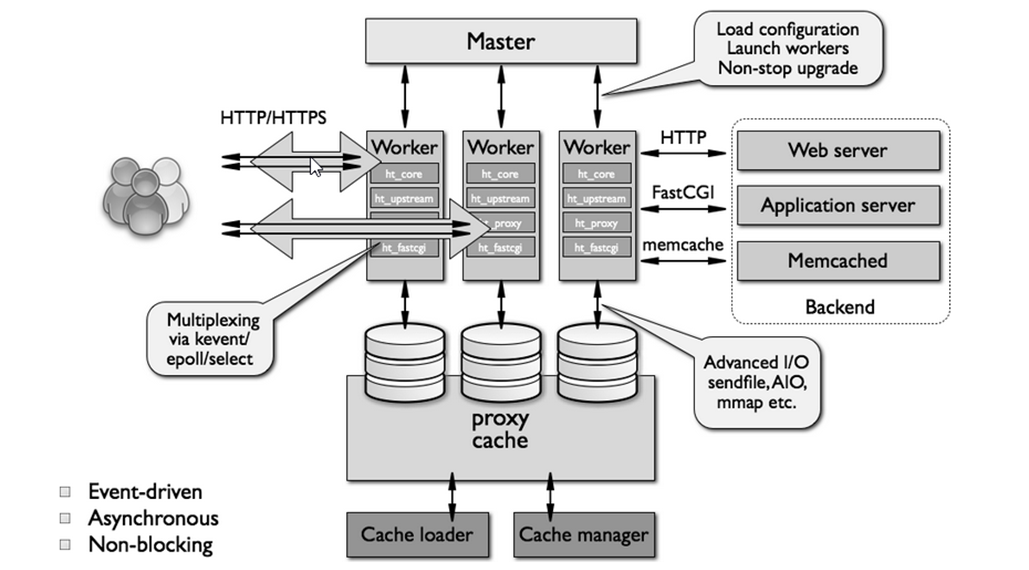
\includegraphics[scale=1]{figuras/nginx-how-it-works} 
\caption{Modelo de funcionamento do Nginx.}
\label{fig:nginx-comofunciona}
\end{figure}

O Nginx é utilizado por vários sítios de grande volume de tráfego como Netflix, GitHub, Pinterest, dentre outros.\\

\section{ApacheBench}
O ApacheBench foi criado em 1996 por Adam Twiss e, posteriormente doado ao Apache \textit{Group}. Originalmente, essa ferramenta foi desenvolvida para verificar o desempenho em servidores HTTP Apache, mas hoje ela é utilizada para fazer testes de desempenho em  praticamente qualquer servidor HTTP.

\section{FastCGI}
Escrever sobre

\section{PHP}
Escrever sobre
\subsection{PHP-FPM}
Escrever sobre
\section{PostgreSQL}
Escrever sobre
\section{VirtualBox}
Escrever sobre
\section{Debian}
Escrever sobre